%!TEX root = ../thesis.tex

\section{実験概要}
前章では, オフライン手法によりend-to-end学習器を用いて, 視覚による経路追従行動を模倣できることを確認した. 前章の実験はシミュレータ上での検証であったが, これを実ロボットに適用する場合, まず画角の広いカメラを3つ用意する. 次に, カメラをロボットの中央及び±0.2[m]に配置して, 経路に沿って走行する. 方向に関しては, 画角の広いカメラで得られた画像から, 目標経路の方向及び±5[deg]回転させた時に得られる画像を切り抜いて, データセットに加える. 各画像に対する目標角速度は, 中央のカメラ画像とペアになる角速度にオフセットを加えて得ることができる. これにより, オンライン手法では目標経路を複数回周回しなければならなかったものが, 1周すればよいことになる. この手法が有効であるかをシミュレータ上の実験により検証することを本実験の目的とする. 

% \section{提案する手法}
% 本章では, 前項でも述べた条件で実験を行い手法の有効性を検証する. 具体的には, 以下のようにロボット及び学習に使用するデータを変更する. 

% \begin{itemize}
%   \item ロボットに搭載するカメラを1つから3つに増やす
%   \item カメラの画角を120度から130度に広げる
%   \item \figref{Fig:crop}のようにカメラから得られる画像サイズを640×480から694×520に変更\par 画像の中央及び左右にそれぞれ640×480で画像を切り抜いてリサイズ
%   \item 収集した角速度に, 各位置と向きを考慮した画像に対応するようにオフセットを追加\par オフセットの値は\tabref{tb:offset}に示す(オフセットの値は前章の実験を基に決定)
% \end{itemize}

\section{実験装置}
手法の有効性を検証するために, シミュレータを用いた実験を行う. 実験環境は5.2章と同様とし, ロボットモデルには\figref{Fig:turtlebot3_3cam}に示すようなカメラを3つ搭載したTurtlebot3\cite{turtlebot3}を用いた.

\begin{figure}[h]
  \centering
  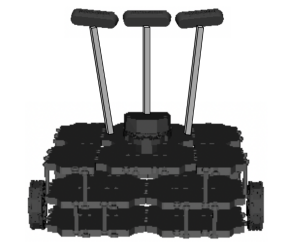
\includegraphics[keepaspectratio, scale=0.5]{images/turtlebot3.png}
  \caption{Turtlebot3 waffle with 3 cameras}
  \label{Fig:turtlebot3_3cam}
\end{figure}

\section{実験方法}
本章では, 上記でも述べた条件で実験を行い手法の有効性を検証する. 

\begin{description}
  \item[1)データ収集]\mbox{}\\ \hspace*{3mm}まず, 学習に使用する角速度について述べる. 角速度は, 収集した角速度に各位置と向きを考慮して, オフセットを加える. オフセットの値は\tabref{tb:offset}に示す. なお, この値はmove\_baseから出力される角速度を参考にしている. \par \hspace*{3mm}次に, カメラ画像に関して述べる. \figref{Fig:add-3cam}のように, ロボットの進行方向と垂直な方向に, 中央のカメラの位置を基準として, ±0.2[m]の位置にカメラを増やし, それぞれの画角を120度から130度に広げる. 画像サイズは640×480から694×520に変更する. また, \figref{Fig:crop}のように画像の中央及び左右にそれぞれ640×480で画像を切り抜いて64×48にリサイズする. 
\end{description}

\begin{table}[h]
  \centering
  \caption{Offsets at each position and orientation}
  \begin{tabular}{|p{2cm}|p{2cm}|p{2cm}|p{2cm}|} \hline
      & 0[m] & 0.2[m] & -0.2[m] \\ \hline
    0[deg] & 0 & -0.2 & 0.2 \\ \hline
    5[deg] & -0.01 & -0.25 & -0.125 \\ \hline
    -5[deg] & 0.01 & 0.125 & 0.25 \\ \hline
  \end{tabular}
  \label{tb:offset}
\end{table}

\newpage
\begin{figure}[h]
  \centering
  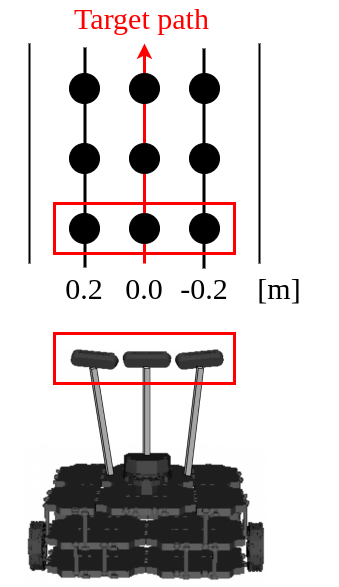
\includegraphics[keepaspectratio, scale=0.31]{images/add_3cam.png}
  \caption{Add cameras at ±0.2[m] along the target path}
  \label{Fig:add-3cam}
\end{figure}

\begin{figure}[h]
  \centering
  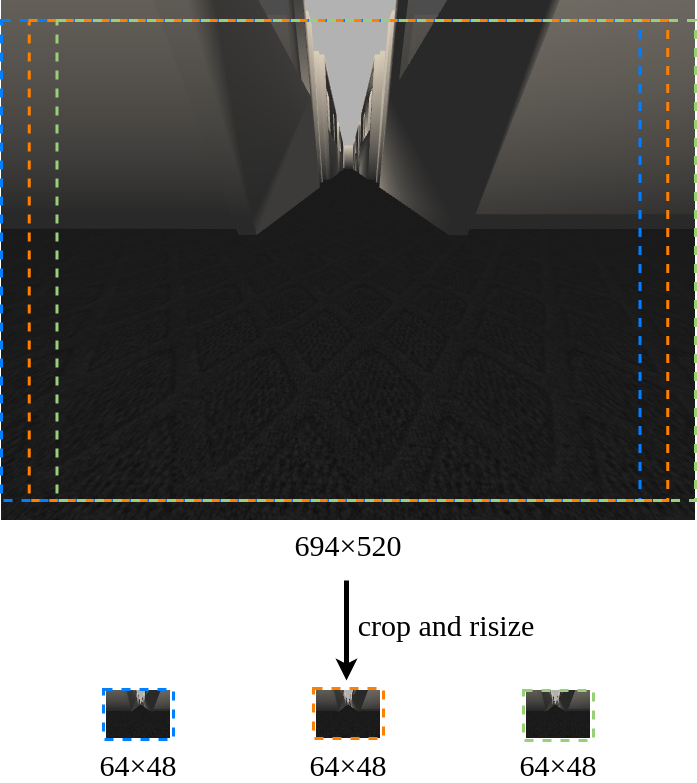
\includegraphics[keepaspectratio, scale=0.28]{images/crop.png}
  \caption{Crop and resize images}
  \label{Fig:crop}
\end{figure}

\newpage
\begin{description}
  \item[2)訓練]\mbox{}\\ \hspace*{3mm}収集したデータを用いて, バッチ学習を4000step行う. 
\end{description}

\begin{description}
  \item[3)テスト]\mbox{}\\ \hspace*{3mm}学習したモデルを用いてロボットを走行させ, \figref{Fig:willow-garage}に示した目標経路を追従できるかを検証する. ロボットの並進速度0.2m/sとし, 経路を1周できた場合を成功とし, 壁に激突した場合を失敗とした. 上記の2)学習と3)テストを30回行い, 経路追従の成功回数を求めた. 
\end{description}

\section{実験結果と考察}
実験結果を\tabref{tb:exp2}に示す. 分母の30は実験回数を示しており, 分子の数は成功回数を示している. 結果的に成功回数は30回中0回となった. テスト時の走行軌跡の一例を\figref{Fig:fail}に示す. 図を見てわかるように, 直進時に左右の壁に衝突して失敗している. また, 目標経路から外れた際に, 復帰するような行動も見られなかった. 教師データとして使用している目標角速度とカメラ画像のどちらか, あるいは両方に原因があるため, 経路追従を継続できないのではないかと考える.\figref{Fig:sample}に, この実験条件で学習したときのlossのグラフを示す. 図から初期でlossが減少に急激して, その後はlossがほぼ変化していないことがわかる. 

\begin{table}[h]
  \centering
  \caption{Number of successes in the experiments of simulator}
  \begin{tabular}{|c|c|} \hline
      Number of successes & 0/30 \\ \hline
    \end{tabular}
  \label{tb:exp2}
\end{table}

\begin{figure}[h]
  \begin{minipage}[b]{0.45\linewidth}
    \centering
    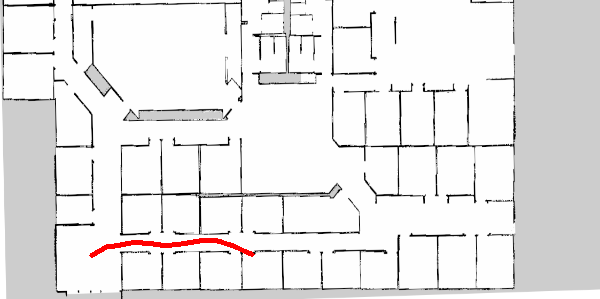
\includegraphics[keepaspectratio, scale=0.35]{images/694_520_0128/traject9.png}
    \subcaption{}
  \end{minipage}
  \begin{minipage}[b]{0.45\linewidth}
    \centering
    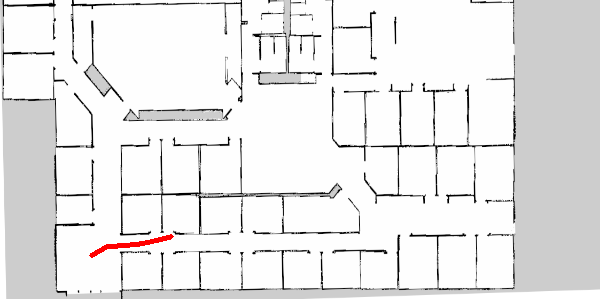
\includegraphics[keepaspectratio, scale=0.35]{images/694_520_0128/traject22.png}
    \subcaption{}
  \end{minipage}
\caption{Example of failed path-tracking}
\label{Fig:fail}
\end{figure}

\newpage
\begin{figure}[h]
  \centering
  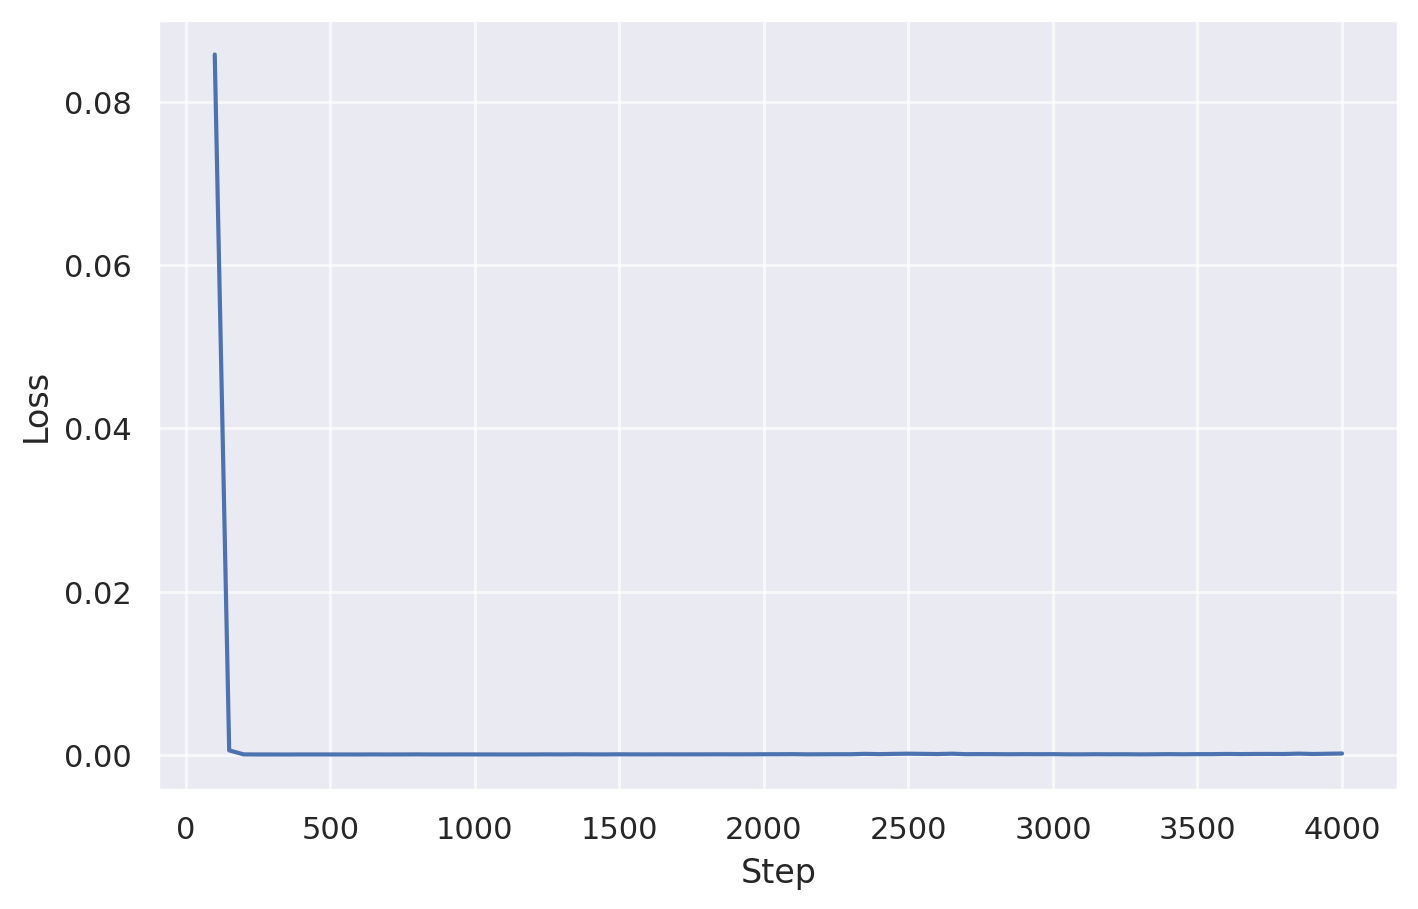
\includegraphics[keepaspectratio, scale=0.6]{images/694_520_9.png}
  \caption{Loss value in the experiment}
  \label{Fig:sample}
\end{figure}

\newpage
\section{まとめ}
本章では, 実環境を想定した実験により, 経路追従行動をオフラインで模倣学習する手法を検討した. シミュレータを用いた実験により, 以下のことを確認した. 

\begin{itemize}
  \item 本条件では, 切り抜いた画像とオフセットを加えた目標角速度を用いた学習では, 経路追従を継続できないことを確認
  \item 目標経路から外れた際に, 復帰するような行動が見られないことを確認
\end{itemize}

% \section{学習に使用した教師データの解析}
% 前章で最も成功率の高かった際の教師データを実験1, 本章の教師データを実験2として比較を行う. これにより, 目標角速度とカメラ画像に問題があるかを調査する. \figref{Fig:ratio}に目標角速度の割合を比較したグラフを示す. 

% \begin{figure}[h]
%   \centering
%   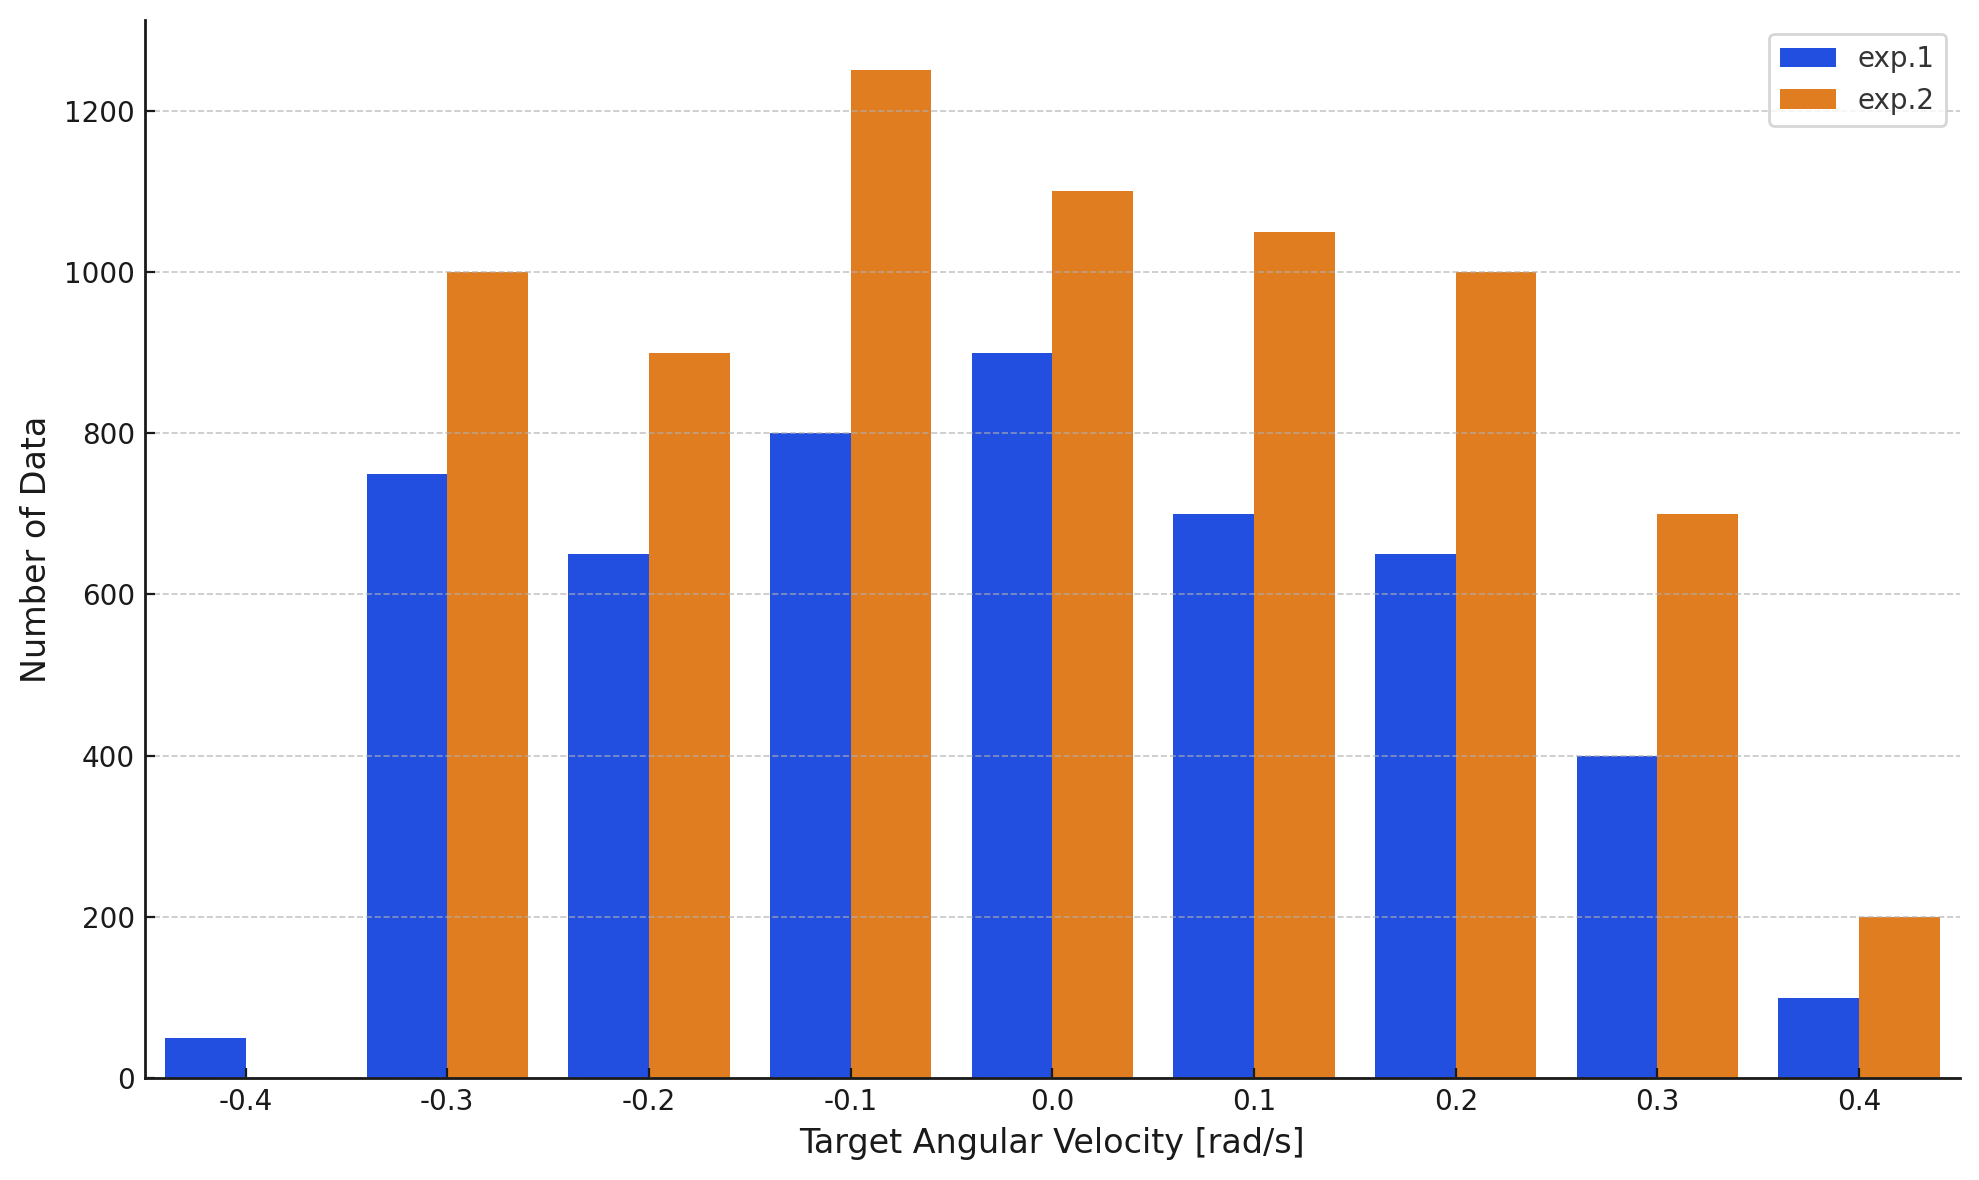
\includegraphics[keepaspectratio, scale=0.5]{images/output.png}
%   \caption{Comparison of target angular velocity ratios}
%   \label{Fig:ratio}
% \end{figure}

% 実験1と実験2の教師データを入れ替えて実験を行った. まず, 実験1のカメラ画像と実験2の目標角速度の組み合わせで学習を行った.